\chapter{Modelling Experiments with SCPs} \label{chp:model}
\section{Overview}
As with any cognitive framework, the most important metric for judging the success of SCPs comes from testing how well SCPs can approximate empirical data across tasks. This chapter will show the suitability of SCPs with a common set of allowable cognitive operations for modelling several well-studied experiments in cognitive modelling.

In particular, we will show that the Wason Selection Task, and Suppression Task and can be modelled at both the general and individual reasoner level with SCPs in a formulation that intuitive and consistent with the WCS approach already described in Chapter~\ref{chp:experiments}.
\section{Suppression Task} \label{sec:supSCP}

\subsection{Suppression Task: WCS}


To model this experiment in the SCP framework, we must first define the SCP Task $\Pi_{sup}=(s_i,M,f(),\gamma)$ which outlines the restrictions and goals of the model. The structure of $s_i$ must be robust enough to capture information regarding a set of rules, variable assignments in the possible world, and conditionals. To this end we define:

\[s_i=\{s_i^\text{el},s_i^\text{elo}\}\]
\[s_i^\text{el}=\{S,\Delta_\text{noSup}, V\} \]
\[s_i^\text{elo}=\{S,\Delta_\text{Sup}, V\} \]




For the the only unconditional rule, that she has an essay to write, we define $S=\{(e \leftarrow \top)\}$. The set of conditional rules $\Delta_{\text{noSup}}=\{l|e\}$ captures the probable assumption that she will study late in the library if she has an essay to write, $\Delta_{\text{sup}}=\{(l|e),(l|o)\}$ captures the addition of the conditional that if the library is open she will study late in the library. And the possible world $V=\{(e,u),(l,u),(o,u)\}$ sets all variable names occurring in $S$ and $\delta$ to unknown.

The second consideration $M$, denotes the set of possible cognitive operations which may occur in the resulting SCPs and realised SCPs of $\Pi_{sup}$. Following the intuition we used in Section~\ref{sec:sup}, we choose cognitive operations that enable application of the WCS and interpretation of conditionals. To that end we define:

\[
M=\{\texttt{addAB}, \texttt{semantic}, \texttt{wc}\}
\]

The external evaluation function should translate the SCP into a decision that can be compared with empirical data. In the Suppression Task we will treat $f_\text{sup}()$ as a function that makes a single choice from the set $\{\text{`she will strudy late in the library'},\text{she will not study late in the library}, \text{we are uncertain if she will study late in the library}\}$. Under the assumption only the final state point $p_n$
determines whether she will study late, we might define $f_\text{sup}()$ as follows:

\begin{algorithm}[H] \label{evaluation:f_sup}
\SetAlgoLined
\SetKwProg{Fn}{Function}{ is}{end}
\Fn{$\texttt{f}_\text{sup}(\pi)$}
{
\tcc{This is a final state evaluation SCP.}
Let $R=[(K[\pi],f())]$ be the set of realised SCPs $r_i=(k,f())$ which can be generated from $\pi$\;
Let $P=[\bar{p}_1,...,\bar{p}_n]$, where $\bar{p}_i$ is the final state of $r_i$\;

$P_\text{el}:=[\bar{p} \in P | \bar{p}[\text{`name'}]=\text{`el'}$\;
$P_\text{elo}:=[\bar{p} \in P | \bar{p}[\text{`name'}]=\text{`elo'}$\;

\uIf {there is a response $\in \texttt{responses}(P_\text{el})$ which is not $\in \texttt{responses}(P_\text{elo})$}
{
\Return 'suppression observed'
}
\Else
{
\Return 'no suppression'
}
}
\Fn{$\texttt{responses}(p)$}
{
\Return $[\texttt{response}(\bar{p}) | \bar{p} \in p]$
}
\Fn{$\texttt{response}(\bar{p})$}
{
\uIf{$I_{\bar{p}(V)}(l)\models \top$}
{
\Return `she will study late in the library'
}
\uElseIf{$I_{\bar{p}(V)}(l)\models \bot$}
{
}
\Else
{
\Return `we are uncertain if she will study late'
}
}

\caption{$\texttt{f}_\text{sup}$}
\end{algorithm}

It is worth noting that one could also define $f_\text{sup}$ in such a way that it iterates over every variable assignment for 'el' and 'elo' in the final state point and sees if any inference is drawn in 'el' that is not drawn in 'elo'. However, the purpose of the external evaluation function is to transform an SCP into an output from the set of empirically observed outputs, and in this case the empirical knowledge is a response to the question ``will she study late in the library?".

Next, we define the empirical result we wish to emulate $\gamma$. In this case we will define $\gamma_\text{noSup}$ to model cases where no suppression is observed, and $\gamma_{\text{sup}}$ to model cases where suppression is observed.
\[\gamma_{\text{noSup}} = \text{no suppression} \]
\[\gamma_{\text{sup}} = \text{suppression observed} \]
Armed with these definitions, it is possible to model the task $\Pi$ as follows:
\[\Pi=(s_i,M,f(),\gamma_{\text{sup}})\]
De Novo search on $\Pi$ returns the satisfying SCP $\mu_\text{sup}$:
\[\mu_\text{sup}=(\pi=(s_i \longmapsto \texttt{addAB} \longmapsto \texttt{wc} \longmapsto \texttt{semantic}),f())\]
Figure~\ref{fig:Suppression_SCP} illustrates the realised SCP for $\mu_\text{sup}$ and illustrates that $\mu_\text{noSup} \models \gamma$. This example has served to show that suppression can modelled in the SCP framework.

\begin{figure}
\centering 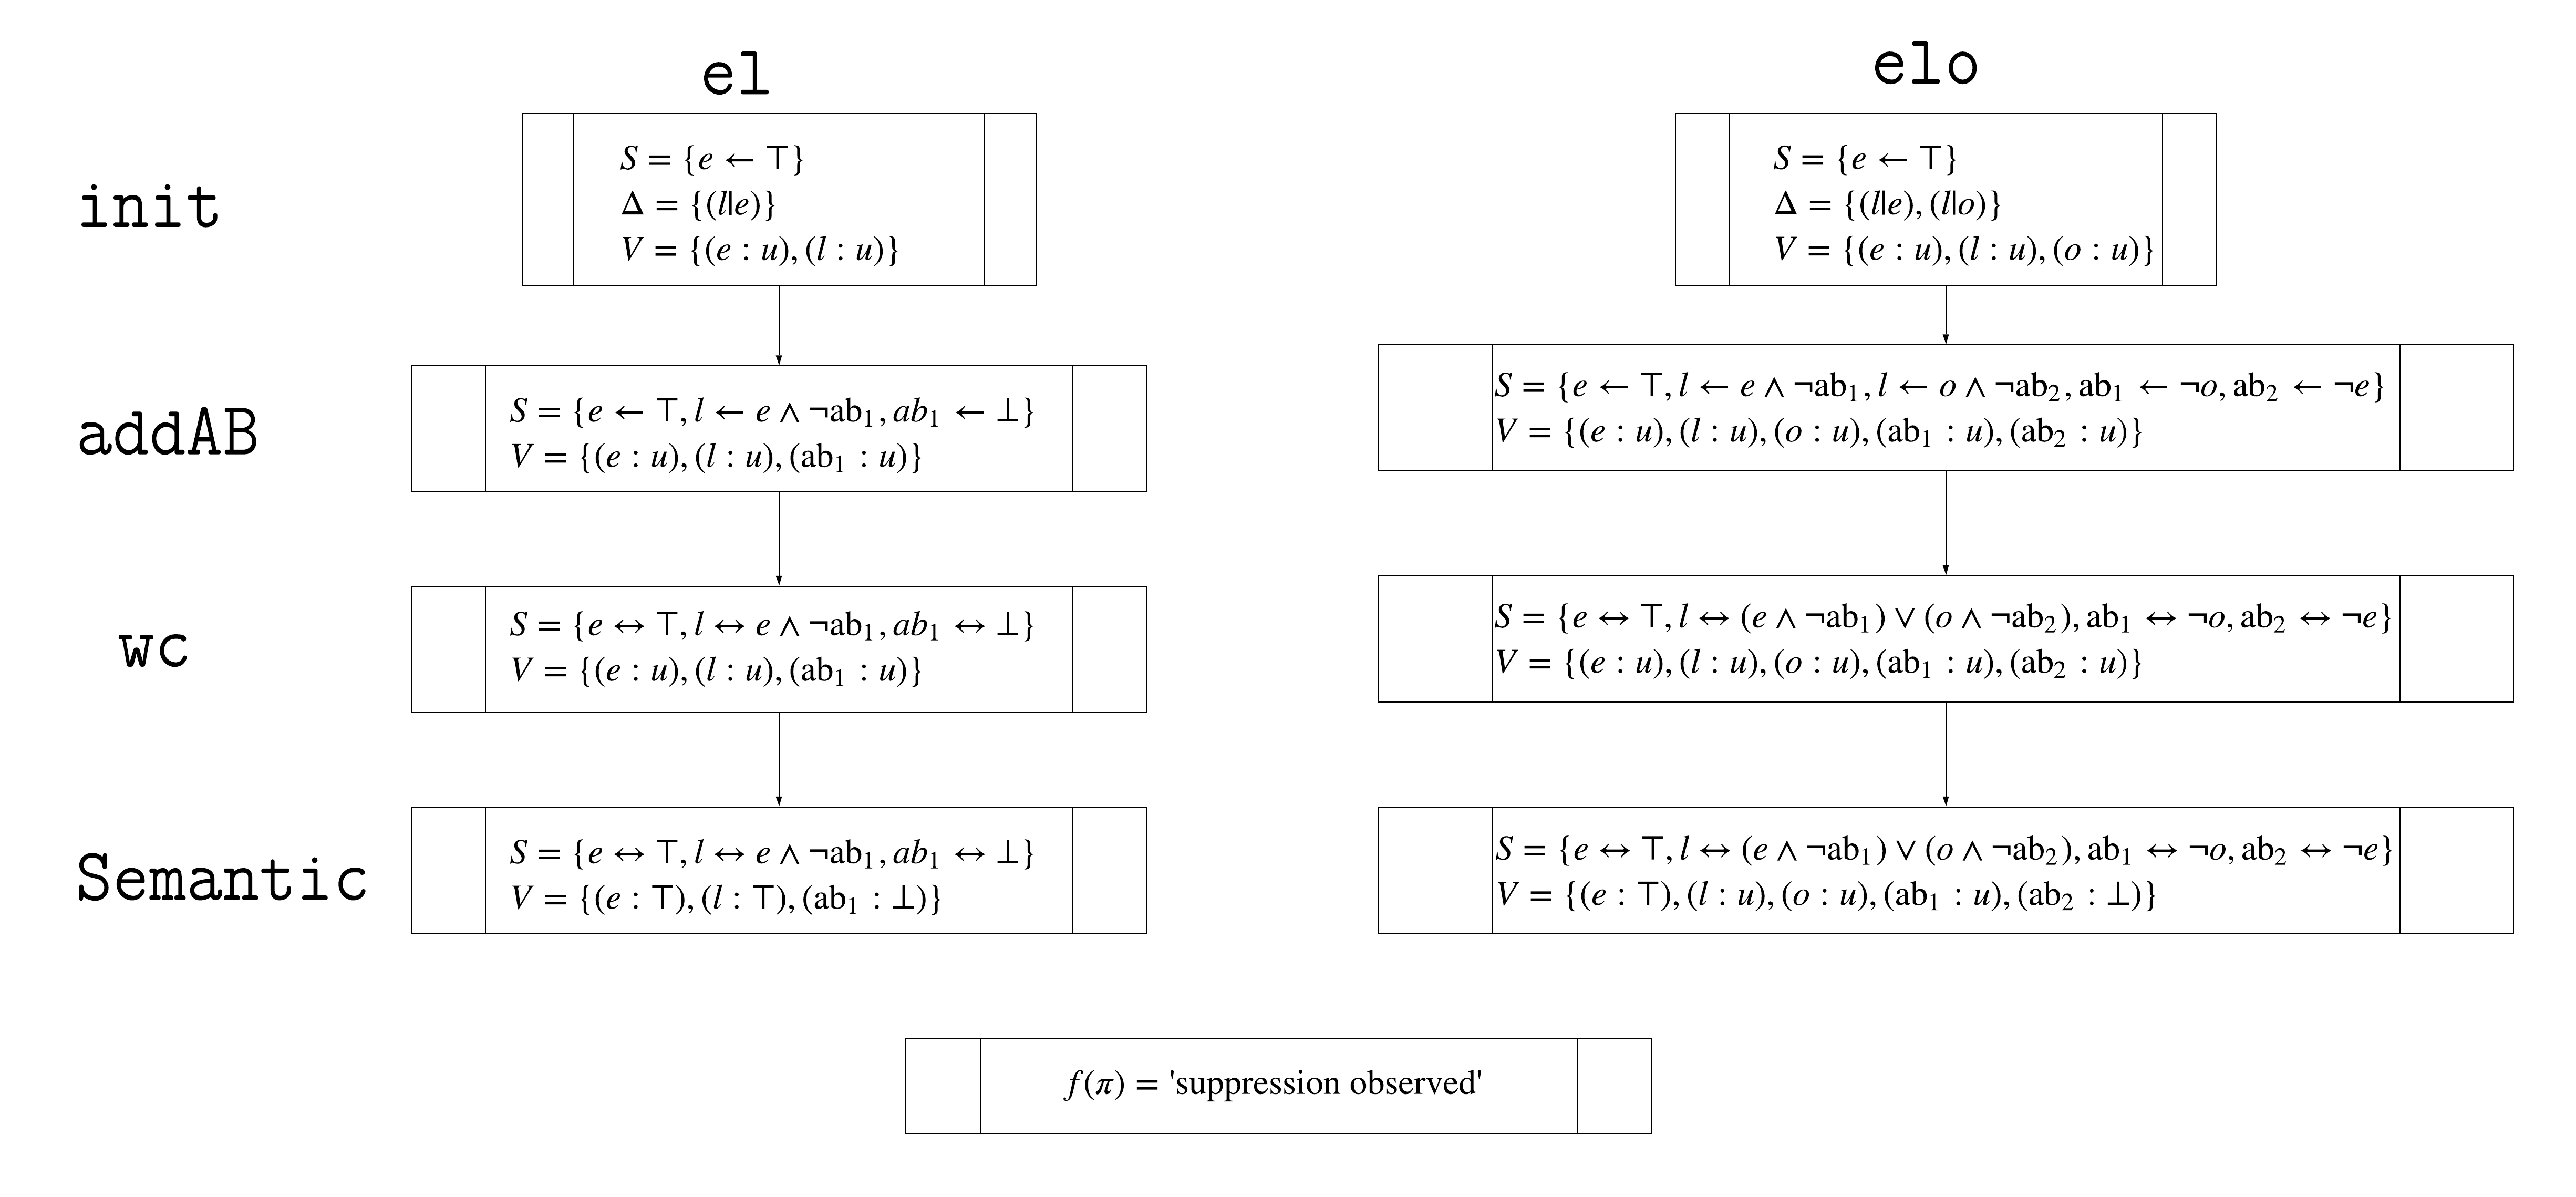
\includegraphics[width=\linewidth]{Suppression_SCP}
\caption{Suppression for the SCP $\mu_\text{sup}=(\pi=(s_i \longmapsto \texttt{addAB} \longmapsto \texttt{wc} \longmapsto \texttt{semantic}),f())$}.
\label{fig:Suppression_SCP}
\end{figure}

%==========================individual reasoners===================================

To illustrate the ability of the framework to model individual reasoners, we examine those reasoners who despite knowing both that if she has an essay to write she will study late in the library and that if the library is open she will study late in the library still do not demonstrate suppression, and instead draw the classical conclusion that she will study late in the library. To this end we define a second SCP Task $\Pi_\text{deviant}$.
\[\Pi_\text{deviant}=(s_i^{\text{sup}},M',f(),\gamma_{\text{noSup}})\]
\[M'=\{\texttt{addAB}, \texttt{semantic}, \texttt{wc}, \texttt{remove}_\bot, \texttt{addExp}\}\]
$M'$ is contains $\texttt{remove}_\bot$ which is able to delete any subset of the variables mentioned in $R[\text{`delete'}]$ of the epistemic state. $\texttt{addExp}$ allows us to add abducible facts to an epistemic state, following the intuition we first used to model the WST in Section~\ref{ssec:wst}. To see the explanations and justifications for these two cognitive operations, refer to Section~\ref{ssec:deletion}, and Section~\ref{ssec:abd}.

Equipped with these two cognitive operations, there are several SCPs which can model $\Pi_\text{deviant}$.

Figure~\ref{fig:Suppression_SCP_del1} shows the realised SCPs for one satisfying SCP for $\Pi_\text{deviant}$. This example shows that deleting the variable $o$ from the epistemic state, prevents suppression from occurring because suppression the abnormality $(\text{ab}_1 \leftarrow \lnot o )$ is the cause of the suppression in $\Pi$, and in $\Pi'$ the abnormality is now given by $(\text{ab}_1 \leftarrow \lnot \top )$.

In the Appendix, Figure~\ref{fig:suppression_python} shows that the non-monotonic cognitive operation \texttt{addExp} can prevent suppression by adding abducibles related to the  free variable $o$.\footnote{The output is too large to graph attractively, and should be viewed in its entirety to confirm that this approach is effective.} This is, as far as I can tell, the first use of \cite{holldobler2015weak}'s abducible approach to the WST to model the Suppression Task. By giving $o$ an assignment, the abnormality $\text{ab}_1\leftrightarrow \lnot o$ no longer evaluates to $u$, and across all responses epistemic states, the `elo' states now model every response \texttt{response} that `el' does.

Both of these examples illustrate the derivation of the classical logical response to the suppression task as a modification of an SCP which did illustrate suppression. This evidences one of the core claims of the SCP Framework which is that it is a reasonable tool for modelling individual reasoners in a cognitive task. 

The value of these examples lies in that they show that classical logic response to a cognitive task is not necessarily derived through the use of classical logic.

\begin{figure}
\centering 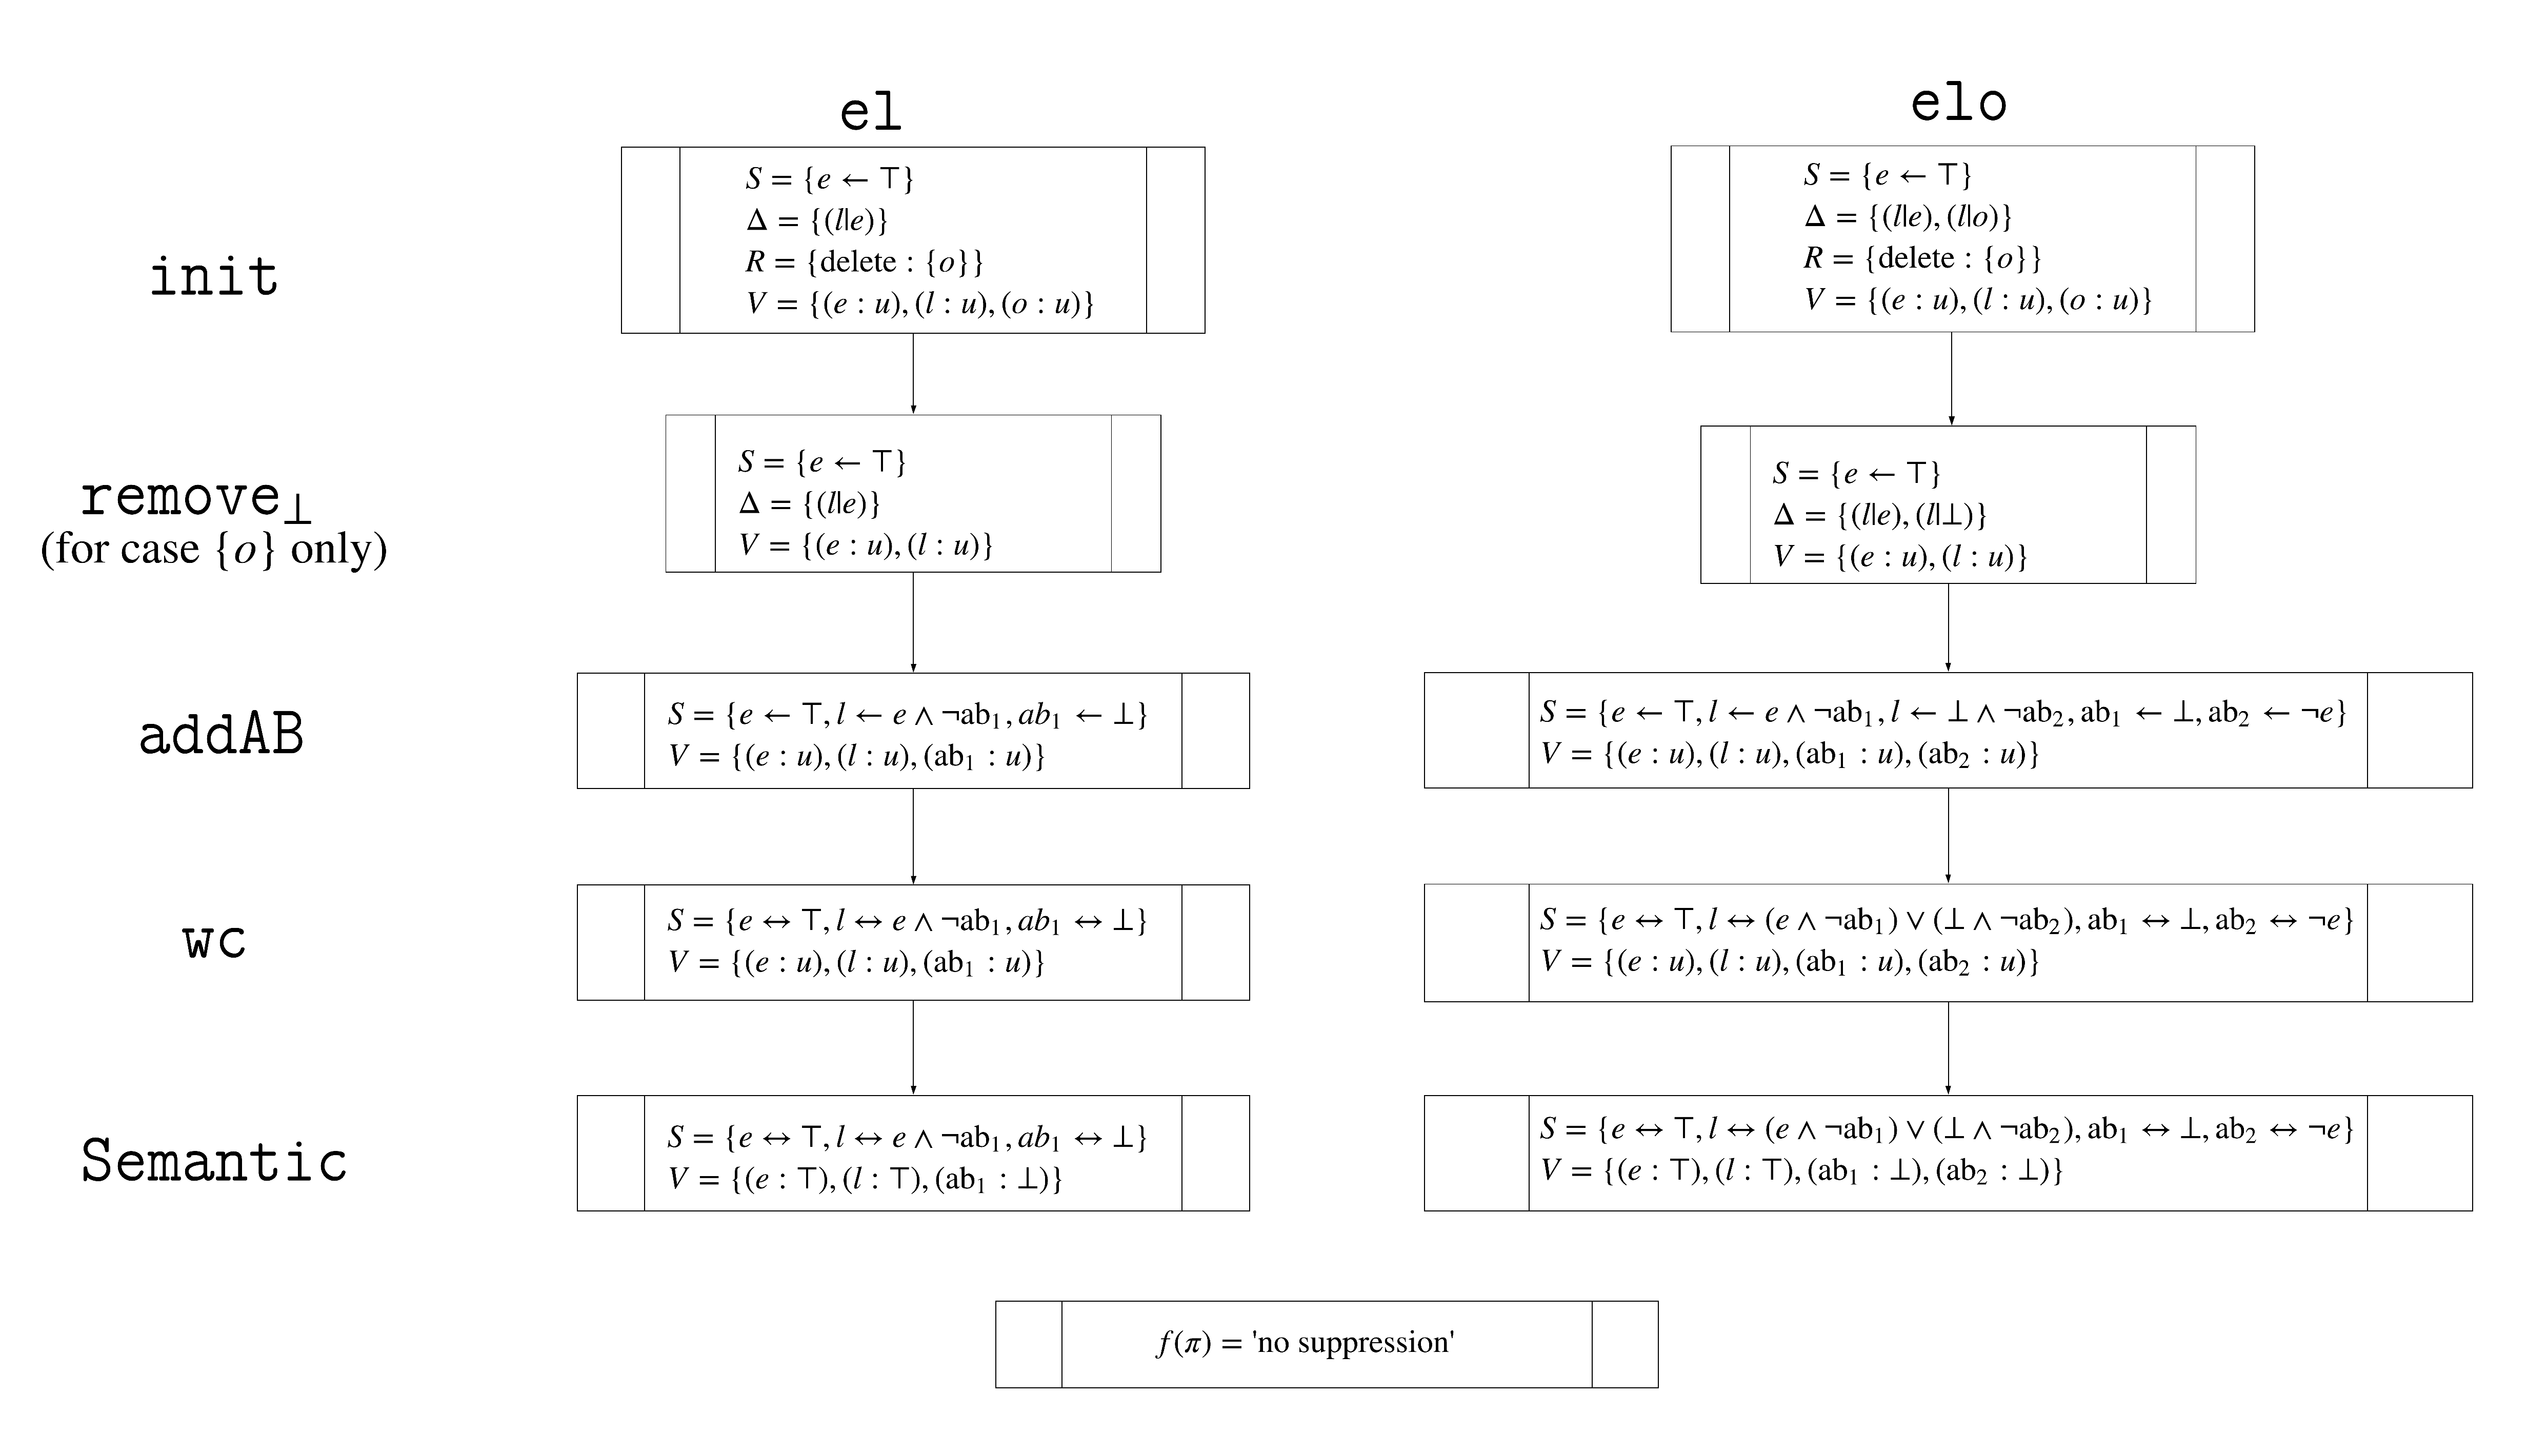
\includegraphics[scale=0.4]{Suppression_SCP_del1}
\caption{Inhibition of Suppression for the SCP $\mu_del=(\pi,f_\text{sup}()), \pi = (s_i \longmapsto \texttt{remove}_\bot \longmapsto \texttt{addAB} \longmapsto \texttt{wc} \longmapsto \texttt{semantic}).$}.
\label{fig:Suppression_SCP_del1}
\end{figure}




\subsection{Suppression Task: Reiter's Default Logic}

As with  Reiter's Default Logic as discussed in Section~\ref{ssec:supReit}, Reiter's Default Logic is not able to model the Suppression Task. This remains the case when using an SCP approximation of this logic. This brief example if provided as evidence that SCPs are able to approximate the Reiter's Default Logic interpretation of the task, rather than to propose any solutions which would make suppression possible.

In order to create this model, we introduce the new cognitive operation $\texttt{I}_W$. $\texttt{I}_W$ interprets the variable $\bar{p}[W]$ of input base point $\bar{p}$, and sets the variables  $\bar{p}[V]$ in a base point $\bar{p}'\in p'$ of the output state point $p'$ to a valid possible world configuration for those variables.


\begin{algorithm}[H] \label{alg:I}
\SetAlgoLined
\SetKwProg{Fn}{Function}{ is}{end}
\Fn{$e$($\bar{p}$)}
{
possibleAss:=$\{w|w$ is a valid possible setting of the variables in $ \bar{p}[V] $ for propositional knowledge base $\bar{p}[W]\}$\;
$p'=\{\}$\;
\For {unique $w \in $ possibleAss}
{
$\bar{p}':=\texttt{clone}(\bar{p})$\;
$\bar{p}'[V]:=w$\;
$p':=p' \cup \bar{p}'$\;
} 
\Return $p'$
}
\caption{$\texttt{I}_w$ generates possible world assignments for a propositional knowledge base $W$.}
\end{algorithm}

Equipped with this new cognitive operation we might define the SCP Task $\Pi_\text{default}$ as follows:
\[\Pi_\text{default}=(s_d,M_d,f_\text{sup}(),\gamma_\text{sup})\]
\[s_d=\{s_d^{el}, s_d^{elo}\}\]
\[s_d^{el}=(W,D_{el},V_{el})\]
\[s_d^{elo}=(W,D_{elo},V_{elo})\]
Where the initial state $s_d$ consists of epistemic states containing the initial information that she will study late in the library, as well as extra conditional information interpreted as defaults, as in Section~\ref{ssec:supReit}, and a possible world variable. Each epistemic state in the initial state point encodes the information required for to form a default theory of the form $(W,D)$.
\[W=\{e\leftarrow \top\}\]
\[
D_{el}=\{\delta_1:\frac{e\leftarrow \top:\text{ab}_1 \leftarrow \bot}{l\leftarrow\top} ,
\delta_2:\frac{\top:\text{ab}_1 \leftarrow \top}{\text{ab}_1\leftarrow\top}
\}
\]
\[
D_{elo}=\{\begin{matrix}\delta_1:\frac{e\leftarrow \top:\text{ab}_1 \leftarrow \bot}{l\leftarrow\top} ,
\delta_2:\frac{o\leftarrow \top:\text{ab}_2 \leftarrow \bot}{l\leftarrow\top},
\delta_3:\frac{o\leftarrow \bot:\text{ab}_1 \leftarrow \top}{\text{ab}_1\leftarrow\top},
\delta_4:\frac{e\leftarrow \bot:\text{ab}_2 \leftarrow \top}{\text{ab}_2\leftarrow\top}
\end{matrix}\}
\]
\[V_{el}=\{(e,u),(l,u)\}\]
\[V_{elo}=\{(e,u),(l,u), (o,u)\}\]
To show the use of SCPs in the default logic interpretation of the suppression task, we limit the set of allowable cognitive operations $M_d$ as follows:
\[M_d=\{\texttt{default},\texttt{I}_w\}\]
De Novo search reveals no satisfying SCPs for $\Pi_\text{default}$, as we would expect from a faithful adaptation of Reiter's Default Logic which is unable to demonstrate suppression. The modified SCP Task $\Pi'_\text{default}=(s_d,M_d,f_\text{sup}(),\gamma_\text{noSup})$, does have a satisfying SCP.

$\mu'_d=(\pi'_d, f_\text{noSup})$.
$\pi'_d=(s_d \longmapsto \texttt{default} \longmapsto \texttt{I}_W)$
We find that suppression is not observed because. We define the final state points of the epistemic states $s_d^{el}$ and $s_d^{elo}$ which we will call $p^{el}$ and $p^{elo}$, respectively. we find that $(l, \top) \in p^{el}_i$, and $(l, \top) \in p^{elo}_j$ for every base point $p^{el}_i \in_S p^{el}$ and $p^{elo}_i \in_S p^{elo}$. These results mimic the intuition and data transformations steps used in Section~\ref{ssec:supReit}, but do so in a more structured. When considered in conjunction with the SCP generated for the WST interpretation of the Suppression Task, the simplicity of the SCP framework for modelling cognitive tasks across different logics is evident.

\section{Wason Selection Task}\label{sec:wstSCP}

\begin{figure}
\centering{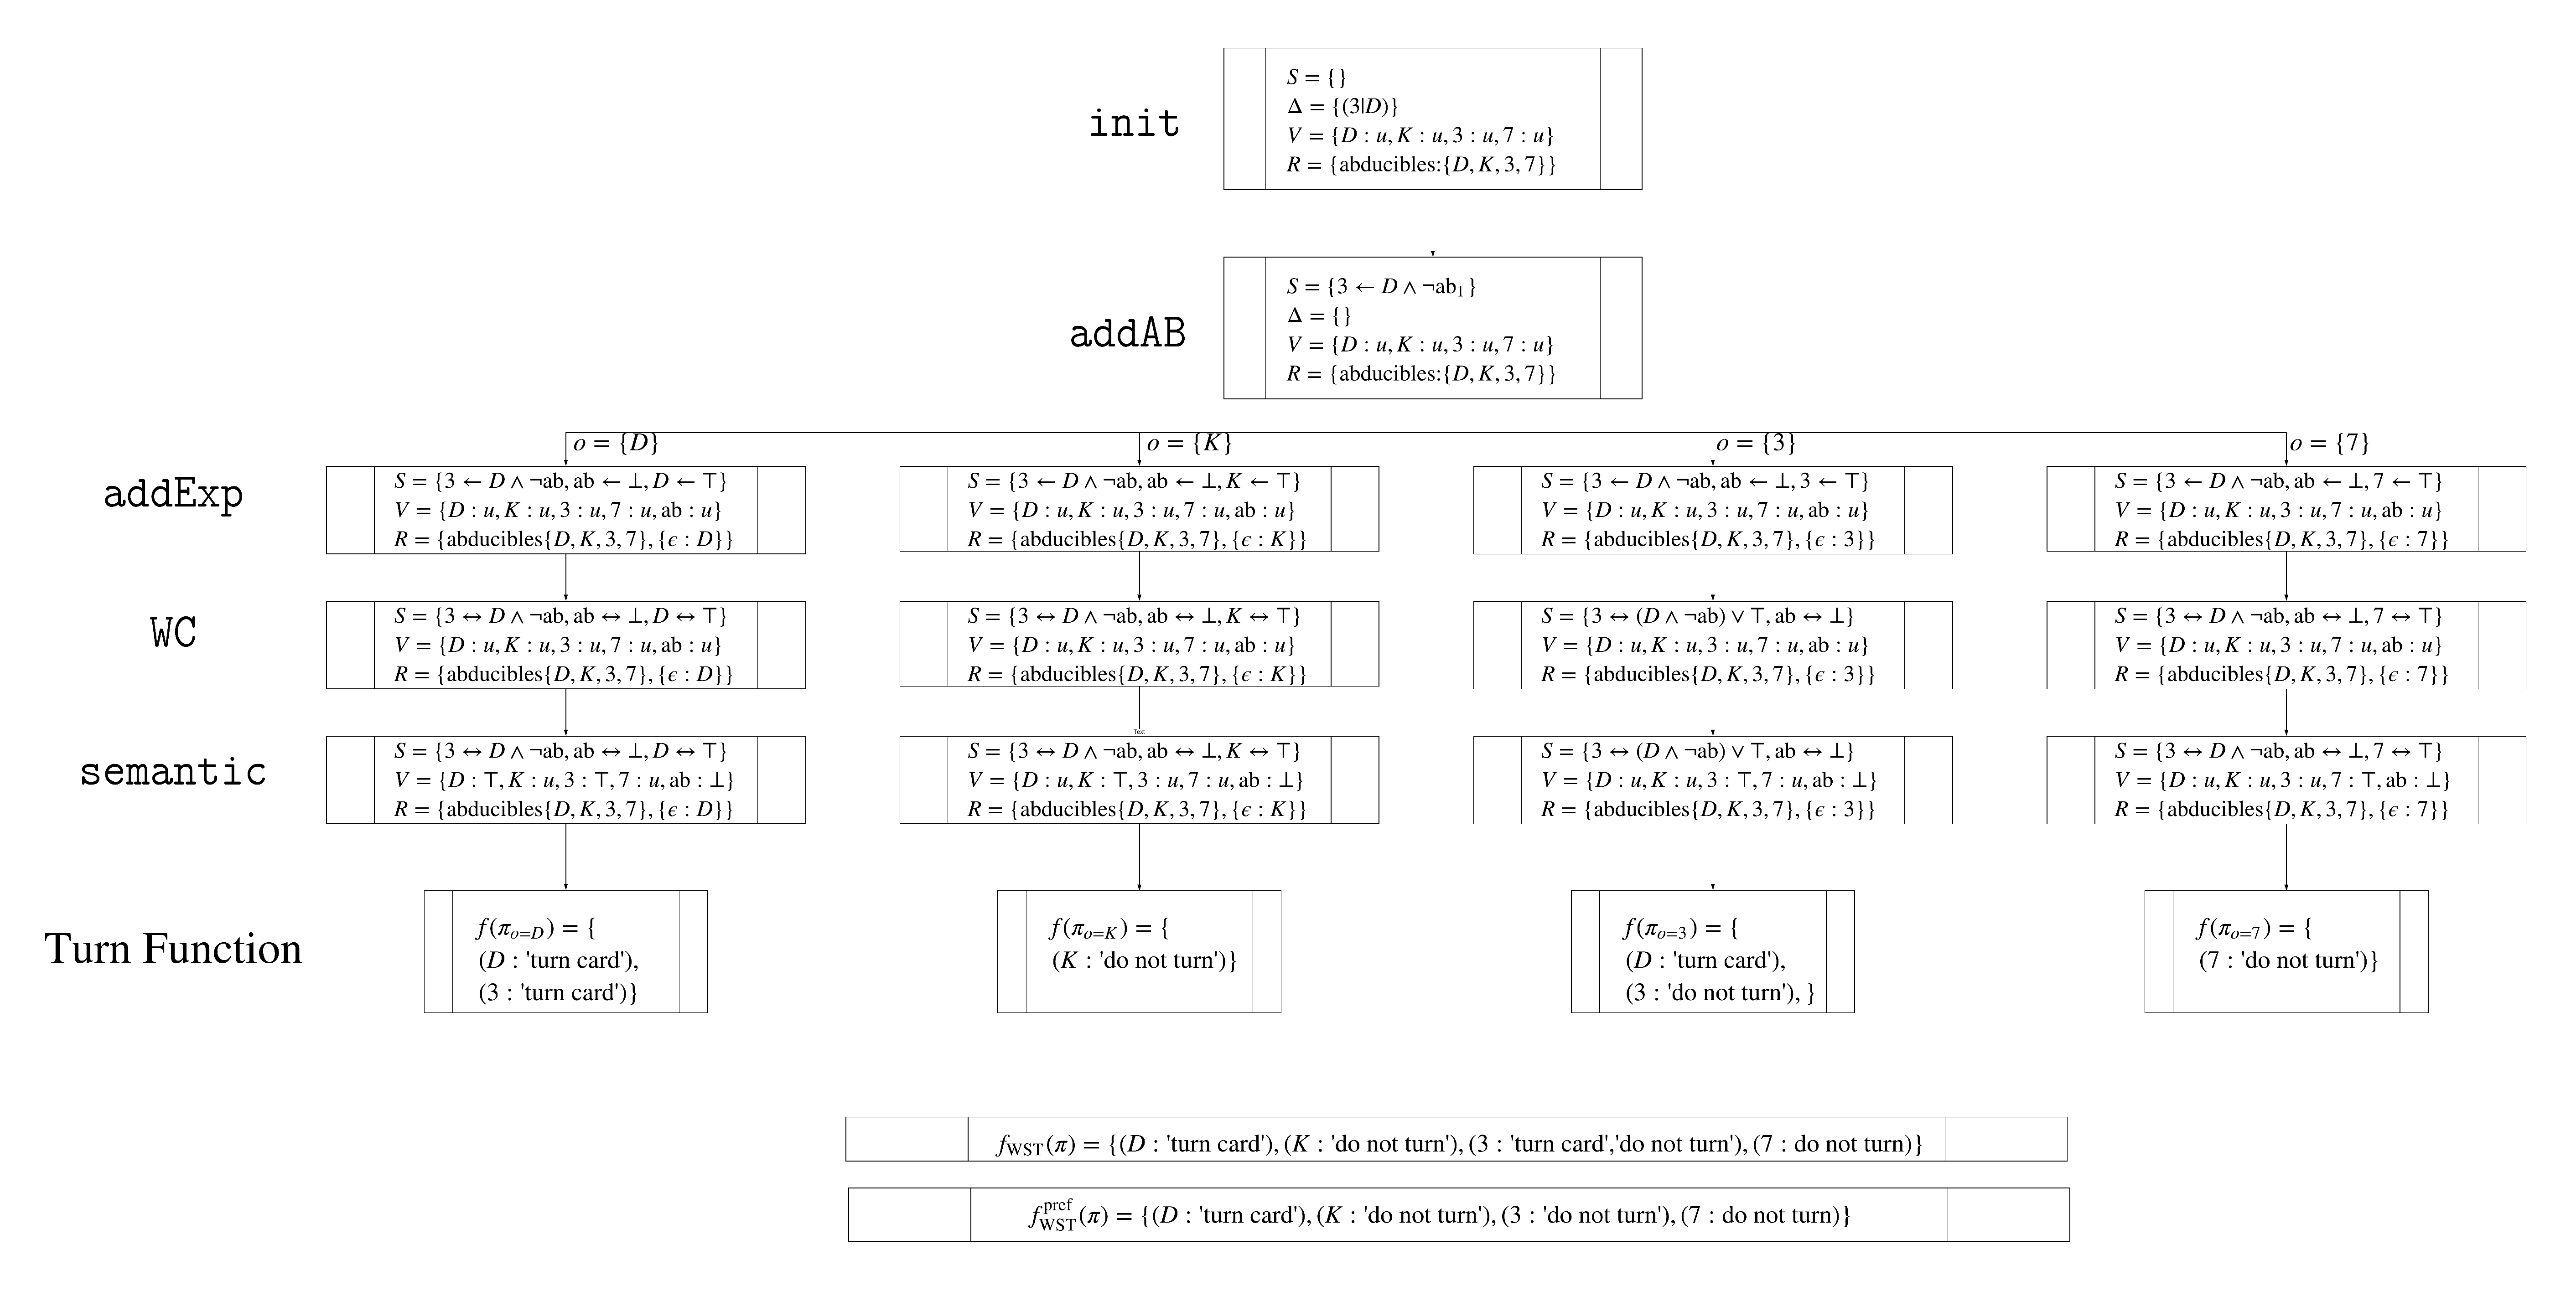
\includegraphics[width=\linewidth]{realisedSCPsWST}}

\caption{Realised SCPs for the SCP interpretation of the WST where $\mu=(\pi_1,f_\text{WST})$, $\pi_1=(s_i \longmapsto \texttt{addAB} \longmapsto \texttt{addExp}  \longmapsto \texttt{wc} \longmapsto \texttt{semantic}))$. Results mimic those observed in \citep{holldobler2015weak}'s WST interpretation.}
\label{fig:rSCP_WST}
\end{figure}

We define the SCP Task $\Pi=(s_i,M,f(),\gamma)$ to model the general case of the WST. The choice of external evaluation function for this task (the turn function), if we are to follow the intuition from Section~\ref{ssec:sup_mod}, has two requirements: it must be able to capture whether an observation $O$ can be explained by the least model of the weakly completed program, and it must ensure that variable assignments which could falsify or verify the conditional rule $(3|D)$ , are present in the least model. 

To this end, we add a set of abducibles to the categorization variable $R$, and combine this with the variables for the set of propositional rules $S$, conditional rules $\Delta$, and possible world $V$ to create the initial state point $s_i$.

Next, we require an intuition for the contents of $s_i$. In this case, abduction can be simulated by the SCP in one of three ways. The first is to create a unique SCP for each possible explanation for each observation as we did for the classical WCS interpretation of the task in Section~\ref{ssec:sup_mod}. But the fact that SCPs may contain an initial state point, rather than just a single epistemic state, enables a more elegant solution that captures the full scope of possible observation, explanation pairings. The other two options are to start with a state point containing each abductive case, or to create cognitive operations which add the abducible cases at computation time. To this end we define:

\[
s_i=(S,\Delta, R)
\]
\[
S=\{\}
\]
\[
\Delta=\{(3|D)\}
\]
\[
R=\{\text{explanations}:\{D\leftarrow \top, D \leftarrow \bot, K\leftarrow \top, K \leftarrow \bot, 3\leftarrow \top, 3 \leftarrow \bot, 7\leftarrow \top, 7\leftarrow \bot\}\}
\]

Because SCPs aim to capture as much cognitive information as possible within the CTM as possible, we will prefer this third case and make use of the categorization variable $R$ to specify both the set of observations, and the possible explanations. The cognitive operation \texttt{AddExp} is created.

For the purposes of readability, we will restrict examination of the abducibles to cases that are of length 1, and contain only positive facts\footnote{A reader wishing to see this process with respect to the full set of abducibles should examine the \texttt{WST.py} file in the SCP implementation.}.

Next, we define the external evaluation function $f_\text{wcs}(\pi)$ as follows:

\begin{algorithm}[H] \label{cogOp:wcs}
\SetAlgoLined
\SetKwProg{Fn}{Function}{ is}{end}
\Fn{$\texttt{f}_\text{WST}(\pi)$}
{
\tcc{This is a final state evaluation SCP.}
Let $R=[(K[\pi],f())]$ be the set of realised SCPs $r_i=(k,f())$ which can be generated from $\pi$\;
Let $P=[p_1,...,p_n]$, where $p_i$ is the final state of $r_i$\;
Let $\eta_i=[\eta_1,...,\eta_n]$, where $\eta_i=p_i[R][\eta]$\;
Let $O=\{(D,\top),(K,\top),(3,\top),(7,\top)\}$ be the set of observations\;
Let $C=\{(3|D), (D' | 7)\}$ be the set of conditionals which must be falsified or verified.\;
Output=\{\}\;
\For{$p_i \in P$}
{
run \texttt{isExplanation}($p_i$)\;
}

\For{each minimal explanation $e$ for observation $o$}
{
\uIf {$I_\text{e[{`V'}]}(C)$ either falsifies or verifies some conditional in $C$}
{
Output[o]:=Output[o]$\cup$ `Turn Card'\;
}
\Else
{
Output[o]:=Output[o]$\cup$ `Do not turn Card'\;
}
}

\Return Output
}
\Fn{$\texttt{isExplanation}(p_i)$}
{
\If{$I_{p_i['V']}(p_i['S']) \models (o \in O)$}
{
\tcc{Then $p_i$ explains $o$.}
Add $p_i$ to the explanations for $o$.
}
}

\caption{$\texttt{f}_\text{WST}$}
\end{algorithm}


Next we create our goals. We will make one goal for each of the canonical cases of the WST. The structure of the goal associates a turn function with every possible observation that needs to be explained.

\[\gamma_{D,3}=\{(\text{D}:\text{turn card}),(\text{3}:\text{turn card}),(\text{K}:\text{turn card}),(\text{7}:\text{do not turn card})\}\]
\[\gamma_{D}=\{(\text{D}:\text{turn card}),(\text{3}:\text{do not turn card}),(\text{K}:\text{turn card}),(\text{7}:\text{do not turn card})\}\]
\[\gamma_{D,7}=\{(\text{D}:\text{turn card}),(\text{3}:\text{do not turn card}),(\text{K}:\text{turn card}),(\text{7}:\text{turn card})\}\]
\[\gamma_{D,3,7}=\{(\text{D}:\text{turn card}),(\text{3}:\text{turn card}),(\text{K}:\text{turn card}),(\text{7}:\text{turn card})\}\]

Next, we define the set of allowable cognitive operations $M$. In this case, because our previous modelling of the general case of the WCS required the addition of explanations from the set of abducibles, we will include the operation \texttt{addExp} (as seen in the SCP Modelling of individual cases of the Suppression Task).

\[M=\{\texttt{addAB}, \texttt{semantic}, \texttt{wc}, \texttt{AddExp}\}\]

The overall planning task, $\Pi$, can now be formulated for the general case of the WST.

\[\Pi=(s_i,M,f_\text{WST}(),\gamma_{D,3})\]

De Novo search for the SCP Plan yields several SCP (differentiated by where the \texttt{addExp} cognitive operation occurs), including this one:

\[\mu_{D,3}=(\pi=(s_i\longmapsto \texttt{addAB} \longmapsto \texttt{addExp} \longmapsto \texttt{wc} \longmapsto \texttt{semantic}),f_\text{WST}())\}\]

\[
f_\text{WST}(\pi)=
\begin{pmatrix}
\{(\text{D}:\{\text{turn card},\text{do not turn})\}, & 
(\text{3}:\{\text{turn card},\text{do not turn})\}, \\
(\text{K}:\{\text{do not turn})\} &
(\text{7}:\{\text{do not turn})\}
\end{pmatrix}
\]



Figure~\ref{fig:rSCP_WST} demonstrates the calculation of $f(\pi)$ for each positive explanation $\eta$ of length 1. When this task is run for minimal explanations of unrestricted length, the set of conclusions for each card returned by $f_\text{WST}()$ do not change. We find that $\mu_{D,3}\models_\text{weak} \gamma_{D,3}$ and that we should turn the cards $D$, and $3$, precisely as in \cite{dietz2014modeling}'s model.

Thus, it has been shown that the SCP Framework is capable of modelling the general response to the abstract case of the WST.

%---------------------------------------Extensions---------------------------------------

In order to model the goals $\gamma_{D}$, $\gamma_{D,7}$, and $\gamma_{D,3,7}$, we must again change our SCP Task. These extensions are easily introduced and, the author hopes, will serve as motivation of the practical and intuitive usefulness of the SCP Framework.

The simplest of these case to model is  $\gamma_{D}$. This could done by creating the new SCP Task $\Pi_D$.

\[
\Pi_D = (s_i, M, \gamma_D, f_\text{WST, simple})
\]

And defining $f_\text{WST, simple}$ precisely as $f_\text{WST}$ was defined, except that the \texttt{isExplanation} function in Algorithm~\ref{alg:outPutcondition} is changed to that of 
Algorithm~\ref{alg:outPutconditionModified}.

\begin{algorithm}[H] \label{alg:outPutcondition}
\SetAlgoLined
\SetKwProg{Fn}{Function}{ is}{end}
\Fn{$\texttt{isExplanation}(p_i)$}
{
\If{$I_{p_i['V']}(p_i['S']) \models (o \in O)$}
{
\tcc{Then $p_i$ explains $o$.}
Add $p_i$ to the explanations for $o$.
}
}
\caption{\texttt{isExplanation} function as it appears in $\texttt{f}_\text{WST}$.}
\end{algorithm}

\begin{algorithm}[H] \label{alg:outPutconditionModified}
\SetAlgoLined
\SetKwProg{Fn}{Function}{ is}{end}
\Fn{$\texttt{isExplanation}(p_i)$}
{
\tcc{We no require that the observation being explained is an element of the proposed explanations.}
\If{$I_{p_i['V']}(p_i['S']) \models (o \in O)$ \textbf{AND} $o \in p_i[R][\epsilon]$}
{
\tcc{Then $p_i$ explains $o$.}
Add $p_i$ to the explanations for $o$.
}
}
\caption{\texttt{isExplanation} function as it appears in $\texttt{f}_\text{WST, simple}$.}
\end{algorithm}

This approach mimics the logic we used to create the Simple WCS Extension in Section~\ref{sec:sup}. However, there is an alternative approach which I prefer. 

One should note that, while $\mu_{D,3}\models_\text{weak} \gamma_{D,3}$, it is also the case that that `do not turn' $\in f_\text{sup}(\pi)[K]$, $f_\text{sup}(\pi)[D]$, and $ f_\text{sup}(\pi)[7]$, but is not in $ f_\text{sup}(\pi)[D]$. If we treat $f_\text{sup}(\pi)$ sceptically and assume that we only turn a card if there is \textit{no reason not to turn it}, we arrive at the conclusion that only $D$ should be turned.

We define a set of preferred responses which prefers the `do not turn' response as follows (using prefered responses as defined in Section~\ref{ssec:f}):
\[
\text{pred}=\{(\text{D}:\text{do not turn}),(\text{3}:\text{do not turn}),(\text{K}:\text{do not turn}),(\text{7}:\text{do not turn})\}
\]


\[
p(f_\text{WST}(\pi),\text{pred})=\{(\text{D}:\text{turn card}),(\text{3}:\text{do not turn}),(\text{K}:\text{do not turn}),(\text{7}:\text{do not turn})\}
\]

Now it is clear that $p(f_\text{WST}(\pi),\text{pred})\models \gamma_D$. To return this to an acceptable SCP format, we may simply define $f_\text{WST}^\text{pref}=p(f_\text{WST}(\pi)$ and observe that $f_\text{WST}^\text{pref}\models \gamma_D$ for SCP $\mu_D=(\pi, f_\text{WST}^\text{pref}())$.
%------------------Contraposition-----------------------------------
Implementing contraposition in the SCP framework we have defined is surprisingly simple. We simply need to define a new plan $\Pi_\text{D,3,7}$ as follows:
\[
\Pi_\text{D,3,7} = (s_i', M, \gamma_{D,3,7}, f_\text{WST}())
\]
\[
s_i'=(S', \Delta', R)
\]
\[
S'=\{(D \leftarrow \lnot D')\}
\]
\[
\Delta'=\{(3|D),(D'|7)\}
\]

Simply by adding the contrapositive conditional and its variable initialization, search returns an SCP $\mu_{D,3,7}=(\pi', f_\text{WST}())$, with $f_\text{WST}(\pi')\models_\text{weak} \gamma_{D,3,7}$. %Figure~@TODO illustrates this fact for positive explanations of length 1.

Finally, the case where the $D$ and $7$ cards are turned (the classical inference), can be modelled by combining aspects of the SCPs above. We define the SCP Plan $\Pi_\text{D,7}$:


\[
\Pi_\text{D,7} = (s_i', M, f_\text{WST}^\text{pref}(), \gamma_{D,7})
\]

And running De Novo search over this Task reveals that the SCP $\mu_{D,7}=(\pi, f_\text{WST}^\text{pref}())$ is a satisfying SCP for the goal $\gamma_{D,7}$. %Figure~@TODO illustrates this point.

Thus, it has been shown that two CTMs $\pi$, and $\pi'$, in conjunction with the external activation functions $f_\text{WST}()$ and $f_\text{WST}^\text{pref}()$ are able to model individual reasoners in the Wason Selection Task.













